%%*************************************************************************
%% Legal Notice:
%% This code is offered as-is without any warranty either expressed or
%% implied; without even the implied warranty of MERCHANTABILITY or
%% FITNESS FOR A PARTICULAR PURPOSE! 
%% User assumes all risk.
%% In no event shall IEEE or any contributor to this code be liable for
%% any damages or losses, including, but not limited to, incidental,
%% consequential, or any other damages, resulting from the use or misuse
%% of any information contained here.
%%
%% All comments are the opinions of their respective authors and are not
%% necessarily endorsed by the IEEE.
%%
%% This work is distributed under the LaTeX Project Public License (LPPL)
%% ( http://www.latex-project.org/ ) version 1.3, and may be freely used,
%% distributed and modified. A copy of the LPPL, version 1.3, is included
%% in the base LaTeX documentation of all distributions of LaTeX released
%% 2003/12/01 or later.
%% Retain all contribution notices and credits.
%% ** Modified files should be clearly indicated as such, including  **
%% ** renaming them and changing author support contact information. **
%%
%% File list of work: IEEEtran.cls, IEEEtran_HOWTO.pdf, bare_adv.tex,
%%                    bare_conf.tex, bare_jrnl.tex, bare_jrnl_compsoc.tex
%%*************************************************************************

% Note that the a4paper option is mainly intended so that authors in
% countries using A4 can easily print to A4 and see how their papers will
% look in print - the typesetting of the document will not typically be
% affected with changes in paper size (but the bottom and side margins will).
% Use the testflow package mentioned above to verify correct handling of
% both paper sizes by the user's LaTeX system.
%
% Also note that the "draftcls" or "draftclsnofoot", not "draft", option
% should be used if it is desired that the figures are to be displayed in
% draft mode.
%
\documentclass[conference]{IEEEtran}

% *** MISC UTILITY PACKAGES ***
%
\usepackage{ifpdf}
% Heiko Oberdiek's ifpdf.sty is very useful if you need conditional
% compilation based on whether the output is pdf or dvi.
% usage:
% \ifpdf
%   % pdf code
% \else
%   % dvi code
% \fi
% The latest version of ifpdf.sty can be obtained from:
% http://www.ctan.org/tex-archive/macros/latex/contrib/oberdiek/
% Also, note that IEEEtran.cls V1.7 and later provides a builtin
% \ifCLASSINFOpdf conditional that works the same way.
% When switching from latex to pdflatex and vice-versa, the compiler may
% have to be run twice to clear warning/error messages.

\usepackage{blindtext}
\usepackage{placeins}
\usepackage{graphicx}
\usepackage{epstopdf}

% use color package to make todos jump out in text
\usepackage{color}
% macro for todo entries addition
\newcommand{\addtodo}[1]{\textcolor{red}{[[#1]]}}

\definecolor{light-gray}{gray}{0.75}
\newcommand{\dummytext}{\textcolor{light-gray}{\Blindtext}}


% *** CITATION PACKAGES ***
%
%\usepackage{cite}
% cite.sty was written by Donald Arseneau
% V1.6 and later of IEEEtran pre-defines the format of the cite.sty package
% \cite{} output to follow that of IEEE. Loading the cite package will
% result in citation numbers being automatically sorted and properly
% "compressed/ranged". e.g., [1], [9], [2], [7], [5], [6] without using
% cite.sty will become [1], [2], [5]--[7], [9] using cite.sty. cite.sty's
% \cite will automatically add leading space, if needed. Use cite.sty's
% noadjust option (cite.sty V3.8 and later) if you want to turn this off.
% cite.sty is already installed on most LaTeX systems. Be sure and use
% version 4.0 (2003-05-27) and later if using hyperref.sty. cite.sty does
% not currently provide for hyperlinked citations.
% The latest version can be obtained at:
% http://www.ctan.org/tex-archive/macros/latex/contrib/cite/
% The documentation is contained in the cite.sty file itself.






% *** GRAPHICS RELATED PACKAGES ***
%
\ifpdf
  % \usepackage[pdftex]{graphicx}
  % declare the path(s) where your graphic files are
  % \graphicspath{{../pdf/}{../jpeg/}}
  % and their extensions so you won't have to specify these with
  % every instance of \includegraphics
  % \DeclareGraphicsExtensions{.pdf,.jpeg,.png}
\else
  % or other class option (dvipsone, dvipdf, if not using dvips). graphicx
  % will default to the driver specified in the system graphics.cfg if no
  % driver is specified.
  % \usepackage[dvips]{graphicx}
  % declare the path(s) where your graphic files are
  % \graphicspath{{../eps/}}
  % and their extensions so you won't have to specify these with
  % every instance of \includegraphics
  % \DeclareGraphicsExtensions{.eps}
\fi
% graphicx was written by David Carlisle and Sebastian Rahtz. It is
% required if you want graphics, photos, etc. graphicx.sty is already
% installed on most LaTeX systems. The latest version and documentation can
% be obtained at: 
% http://www.ctan.org/tex-archive/macros/latex/required/graphics/
% Another good source of documentation is "Using Imported Graphics in
% LaTeX2e" by Keith Reckdahl which can be found as epslatex.ps or
% epslatex.pdf at: http://www.ctan.org/tex-archive/info/
%
% latex, and pdflatex in dvi mode, support graphics in encapsulated
% postscript (.eps) format. pdflatex in pdf mode supports graphics
% in .pdf, .jpeg, .png and .mps (metapost) formats. Users should ensure
% that all non-photo figures use a vector format (.eps, .pdf, .mps) and
% not a bitmapped formats (.jpeg, .png). IEEE frowns on bitmapped formats
% which can result in "jaggedy"/blurry rendering of lines and letters as
% well as large increases in file sizes.
%
% You can find documentation about the pdfTeX application at:
% http://www.tug.org/applications/pdftex





% *** MATH PACKAGES ***
%
%\usepackage[cmex10]{amsmath}
% A popular package from the American Mathematical Society that provides
% many useful and powerful commands for dealing with mathematics. If using
% it, be sure to load this package with the cmex10 option to ensure that
% only type 1 fonts will utilized at all point sizes. Without this option,
% it is possible that some math symbols, particularly those within
% footnotes, will be rendered in bitmap form which will result in a
% document that can not be IEEE Xplore compliant!
%
% Also, note that the amsmath package sets \interdisplaylinepenalty to 10000
% thus preventing page breaks from occurring within multiline equations. Use:
%\interdisplaylinepenalty=2500
% after loading amsmath to restore such page breaks as IEEEtran.cls normally
% does. amsmath.sty is already installed on most LaTeX systems. The latest
% version and documentation can be obtained at:
% http://www.ctan.org/tex-archive/macros/latex/required/amslatex/math/





% *** SPECIALIZED LIST PACKAGES ***
%
%\usepackage{algorithmic}
% algorithmic.sty was written by Peter Williams and Rogerio Brito.
% This package provides an algorithmic environment fo describing algorithms.
% You can use the algorithmic environment in-text or within a figure
% environment to provide for a floating algorithm. Do NOT use the algorithm
% floating environment provided by algorithm.sty (by the same authors) or
% algorithm2e.sty (by Christophe Fiorio) as IEEE does not use dedicated
% algorithm float types and packages that provide these will not provide
% correct IEEE style captions. The latest version and documentation of
% algorithmic.sty can be obtained at:
% http://www.ctan.org/tex-archive/macros/latex/contrib/algorithms/
% There is also a support site at:
% http://algorithms.berlios.de/index.html
% Also of interest may be the (relatively newer and more customizable)
% algorithmicx.sty package by Szasz Janos:
% http://www.ctan.org/tex-archive/macros/latex/contrib/algorithmicx/




% *** ALIGNMENT PACKAGES ***
%
%\usepackage{array}
% Frank Mittelbach's and David Carlisle's array.sty patches and improves
% the standard LaTeX2e array and tabular environments to provide better
% appearance and additional user controls. As the default LaTeX2e table
% generation code is lacking to the point of almost being broken with
% respect to the quality of the end results, all users are strongly
% advised to use an enhanced (at the very least that provided by array.sty)
% set of table tools. array.sty is already installed on most systems. The
% latest version and documentation can be obtained at:
% http://www.ctan.org/tex-archive/macros/latex/required/tools/


%\usepackage{mdwmath}
%\usepackage{mdwtab}
% Also highly recommended is Mark Wooding's extremely powerful MDW tools,
% especially mdwmath.sty and mdwtab.sty which are used to format equations
% and tables, respectively. The MDWtools set is already installed on most
% LaTeX systems. The lastest version and documentation is available at:
% http://www.ctan.org/tex-archive/macros/latex/contrib/mdwtools/


% IEEEtran contains the IEEEeqnarray family of commands that can be used to
% generate multiline equations as well as matrices, tables, etc., of high
% quality.


%\usepackage{eqparbox}
% Also of notable interest is Scott Pakin's eqparbox package for creating
% (automatically sized) equal width boxes - aka "natural width parboxes".
% Available at:
% http://www.ctan.org/tex-archive/macros/latex/contrib/eqparbox/





% *** SUBFIGURE PACKAGES ***
%\usepackage[tight,footnotesize]{subfigure}
% subfigure.sty was written by Steven Douglas Cochran. This package makes it
% easy to put subfigures in your figures. e.g., "Figure 1a and 1b". For IEEE
% work, it is a good idea to load it with the tight package option to reduce
% the amount of white space around the subfigures. subfigure.sty is already
% installed on most LaTeX systems. The latest version and documentation can
% be obtained at:
% http://www.ctan.org/tex-archive/obsolete/macros/latex/contrib/subfigure/
% subfigure.sty has been superceeded by subfig.sty.



%\usepackage[caption=false]{caption}
%\usepackage[font=footnotesize]{subfig}
% subfig.sty, also written by Steven Douglas Cochran, is the modern
% replacement for subfigure.sty. However, subfig.sty requires and
% automatically loads Axel Sommerfeldt's caption.sty which will override
% IEEEtran.cls handling of captions and this will result in nonIEEE style
% figure/table captions. To prevent this problem, be sure and preload
% caption.sty with its "caption=false" package option. This is will preserve
% IEEEtran.cls handing of captions. Version 1.3 (2005/06/28) and later 
% (recommended due to many improvements over 1.2) of subfig.sty supports
% the caption=false option directly:
%\usepackage[caption=false,font=footnotesize]{subfig}
%
% The latest version and documentation can be obtained at:
% http://www.ctan.org/tex-archive/macros/latex/contrib/subfig/
% The latest version and documentation of caption.sty can be obtained at:
% http://www.ctan.org/tex-archive/macros/latex/contrib/caption/




% *** FLOAT PACKAGES ***
%
%\usepackage{fixltx2e}
% fixltx2e, the successor to the earlier fix2col.sty, was written by
% Frank Mittelbach and David Carlisle. This package corrects a few problems
% in the LaTeX2e kernel, the most notable of which is that in current
% LaTeX2e releases, the ordering of single and double column floats is not
% guaranteed to be preserved. Thus, an unpatched LaTeX2e can allow a
% single column figure to be placed prior to an earlier double column
% figure. The latest version and documentation can be found at:
% http://www.ctan.org/tex-archive/macros/latex/base/



%\usepackage{stfloats}
% stfloats.sty was written by Sigitas Tolusis. This package gives LaTeX2e
% the ability to do double column floats at the bottom of the page as well
% as the top. (e.g., "\begin{figure*}[!b]" is not normally possible in
% LaTeX2e). It also provides a command:
%\fnbelowfloat
% to enable the placement of footnotes below bottom floats (the standard
% LaTeX2e kernel puts them above bottom floats). This is an invasive package
% which rewrites many portions of the LaTeX2e float routines. It may not work
% with other packages that modify the LaTeX2e float routines. The latest
% version and documentation can be obtained at:
% http://www.ctan.org/tex-archive/macros/latex/contrib/sttools/
% Documentation is contained in the stfloats.sty comments as well as in the
% presfull.pdf file. Do not use the stfloats baselinefloat ability as IEEE
% does not allow \baselineskip to stretch. Authors submitting work to the
% IEEE should note that IEEE rarely uses double column equations and
% that authors should try to avoid such use. Do not be tempted to use the
% cuted.sty or midfloat.sty packages (also by Sigitas Tolusis) as IEEE does
% not format its papers in such ways.





% *** PDF, URL AND HYPERLINK PACKAGES ***
%
%\usepackage{url}
% url.sty was written by Donald Arseneau. It provides better support for
% handling and breaking URLs. url.sty is already installed on most LaTeX
% systems. The latest version can be obtained at:
% http://www.ctan.org/tex-archive/macros/latex/contrib/misc/
% Read the url.sty source comments for usage information. Basically,
% \url{my_url_here}.





% *** Do not adjust lengths that control margins, column widths, etc. ***
% *** Do not use packages that alter fonts (such as pslatex).         ***
% There should be no need to do such things with IEEEtran.cls V1.6 and later.
% (Unless specifically asked to do so by the journal or conference you plan
% to submit to, of course. )


% correct bad hyphenation here
\hyphenation{op-tical net-works semi-conduc-tor}


\begin{document}
%
% paper title
% can use linebreaks \\ within to get better formatting as desired
\title{\textbf{Dfuzzer: A D-Bus fuzzing tool}}


% author names and affiliations
% use a multiple column layout for up to three different
% affiliations
\author{\IEEEauthorblockN{Mat\'{u}\v{s} Marfefka and Petr Muller,}
\IEEEauthorblockA{Faculty of Information Technology\\
Brno University of Technology,\\
Bo\v{z}et\v{e}chova 1/2 Brno, Czech Republic}
\IEEEauthorblockA{Red Hat,\\
Purky\v{n}ova 99/75a Brno, Czech Republic}
}
% conference papers do not typically use \thanks and this command
% is locked out in conference mode. If really needed, such as for
% the acknowledgment of grants, issue a \IEEEoverridecommandlockouts
% after \documentclass

% make the title area
\maketitle


\begin{abstract}
Fuzz testing or fuzzing is~a method used for~discovering faults in~software~and
it is an~automated process of~testing computer programs. This method of~testing
provides random or invalid data to~a~computer program inputs and~monitors
exceptions generated by a~program such as crashes or memory leaks.

D-Bus is an~inter-process communication~(IPC) system used and~primary developed
for~the~GNU/Linux operating system. It allows one or more applications
to~communicate with~one~another.

In~order to~fuzz test D-Bus applications Dfuzzer was developed, a~tool which is
capable to~connect to~a~D-Bus daemon and communicate with other processes which
are also connected to~it.
\end{abstract}

\begin{keywords}
D-Bus, fuzzer, fuzzing, testing, automation, pseudo-random data generation, IPC
\end{keywords}

% For peer review papers, you can put extra information on the cover
% page as needed:
% \ifCLASSOPTIONpeerreview
% \begin{center} \bfseries EDICS Category: 3-BBND \end{center}
% \fi
%
% For peerreview papers, this IEEEtran command inserts a page break and
% creates the second title. It will be ignored for other modes.
\IEEEpeerreviewmaketitle



\section{Introduction}
\addtodo{Zbezne popsat co je DBus a jakou hraje roli v Linuxu}
\addtodo{Popsat problem co resime a jeho vyznam}
\addtodo{Pozor, reviewers nemusi byt linux experti}

Testing is used to~find bugs~(errors or other defects) in~software. By~finding bugs,
testing also provides quality assurance of~software. Software testing can be stated
as the~process of~validating and~verifying that a~computer software:
\begin{itemize}
	\item meets the~design and~development requirements,
	\item works as expected,
	\item is secure,
	\item and~that bugs are not present.
\end{itemize}

Fuzzing is a~type of~testing where a~goal is to~find bugs in~software, preferably
ones that have security implications. Fuzzing is automated, brute force technique
of~testing and~it exploits the~fact that many bugs in~software are caused
by~handling inputs from~a~user without applying validation routines on~that
inputs. The~goal of~fuzz testing~(fuzzing) is to~crash an~application or a~protocol
and~analyze the~results.

The~term fuzzing was first used by~professor Barton Miller who used fuzzing to~test
robustness of~UNIX applications in~1989~\cite{Fuzzing2}. Fuzzing is defined
in~``Fuzzing: Brute Force Vulnerability Discovery''~\cite[p.~22]{Fuzzing} as
``\emph{a~method for~discovering faults in~software by~providing unexpected
input and~monitoring for~exceptions. It is typically an~automated or semiautomated
process that involves repeatedly manipulating and~supplying data to~target software
for~processing}''.
Another definition~(from ``Fuzzing for~Software Security Testing and~Quality
Assurance''~\cite[p.~1]{Fuzzing2}) says it is ``\emph{a~highly automated testing
technique that covers numerous boundary cases using invalid data~(from~files,
network protocols, API calls, and~other targets) as application input to~better
ensure the~absence of~exploitable vulnerabilities. The~name comes~from modem
applications tendency to~fail due to~random input caused by~line noise on~`fuzzy'
telephone lines}''.

Fuzzing is close to~the~boundary value analysis, where you create test values that
infringe the~boundary of~known good and~bad values. Fuzzing is very effective
because many exploitable vulnerabilities are caused by~applications accepting
user input and~processing that data without applying validation
routines~\cite{Fuzzing}.

Computers use protocols in~all aspects of~internal and~external communication.
Protocols represent a~structure for~data transfer and~processing with~defined
syntax. Certain standards and~rules understood by~both sending and~receiving
entities must be agreed on~to~communicate data in~meaningful way~\cite{Fuzzing}.
Some protocols are designed to~be human readable and~are represented in~plain
text form. Other protocols are represented in~binary format.

D-Bus is a~binary protocol and~a~message bus system providing applications
a~simple way to~talk to~one another. D-Bus is ``\emph{a~system for~\mbox{inter-process}
communication~(IPC) and~Remote Procedure Calling~(RPC) between
processes running on the same machine and~makes it simple and~reliable to~code
a~`single instance' application or daemon, and~to~launch applications and~daemons
on~demand when their services are needed}''~\cite{DBUS}.

As D-Bus has become important part of~almost all GNU/Linux distribution there
are more and~more applications which use it for~IPC. Fuzzing is ideal for~testing
these applications as they have interfaces which contain callable methods
with~input arguments. In~this paper we present the~Dfuzzer, tool for~fuzz
testing D-Bus applications. It is capable to~test interfaces which applications
export to~the~D-Bus. The~tool is focused on~finding bugs related to~memory leaks
and~buffer overflows by~providing still expanding pseudo-random data and~boundary
values to~applications inputs.

\section{DBus message bus}
\addtodo{Trochu detailneji popsat, co je dbus, ale neprehanet}
D-Bus was created to~provide IPC system with a single, unified protocol
and~currently, it is used as default IPC mechanism for~exhanging data between
applications in~desktop environments as for~example GNOME, KDE or Xfce and~even
Windows port exists. Besides desktop applications communication it is also used
for~communicating between system applications and~user sessions.

D-Bus has both the~system bus daemon (for~events such as ``new hardware device
added'' or ``printer queue changed'') and~the~session bus daemon (for~general
inter-process communication needs among user \mbox{applications}). The~message bus
is built on~top of~a~general one-to-one message passing framework, which can be
used by~any two applications to~communicate directly~(without going through
the~message bus daemon). The~communicating applications are either on~one computer,
or they communicate through unencrypted TCP/IP socket suitable for~use behind
a~firewall~\cite{DBUS}.

D-Bus has several layers:
\begin{itemize}
	\item A~library, \texttt{libdbus}, that allows two applications to~connect
		to~each other and~exchange messages.
	\item A~message bus daemon executable, built on~\texttt{libdbus},
		that multiple applications can connect~to. The daemon can route messages
		from~one application to~zero or more other applications.
	\item Wrapper libraries or bindings based on~particular application frameworks.
\end{itemize}


\begin{figure}[h]
\centering
\caption{D-Bus overview~\cite{DBUS}}
\label{fig:dbus_image}
\includegraphics[width=0.5\textwidth]{dbus_diagram.eps}
\end{figure}


D-Bus contains the~bus daemons which act as~routers for~messages. Processes
can connect to~the~bus daemons to~use their routing services as stated on~D-Bus
overview~\ref{fig:dbus_image}. There are two standard buses: the~system bus
and~the~session bus.\\

The~system bus is a~global daemon that any application running in~any
context can use as~a~transport router. It is a~single point where applications
can export services that anyone can use. Only one system bus daemon
can be run at a~time within~an~operating system.\\

The~session bus is the~bus local to~the~current user's session. It is used
for~communication between applications running within the~same X~Window System\footnote{X~Window is a~system and~a~network protocol that provides a~basis
for~graphical user interfaces} session. For every login to~X, a~session bus
daemon is started.\\

D-BUS protocol is binary, which means D-BUS messages incur low overhead when
marshaling and~demarshaling data. Messages consist of~two sections, the~header
and~the~body. The~header contains routing information and~the~type signature
for~the~data. The body contains the~data being sent in~binary format. Each
piece~of~data has a~type code \mbox{associated} with~it and~is packed into the~body
accordingly. Some common types include bytes, 32 and~64 bit integers, doubles,
unix file descriptors and~strings. Common data types can be used to~build more
complex data~types such as arrays, dictionaries or structures.



%%%%%%%%%%%%%%%%%%%%%%%%%%%%%%%%%%%%%%%%%%%%%%%%%%%%%%%%%%%%%%%%%%%%%%%%
\section{Tool description}
\addtodo{!!!Sepsat selling points!!!}
\addtodo{Tohle by melo byt teziste prace a tvorit vetsinu obsahu}
\addtodo{Archictecture overview}
\subsection{Ballast generation}
\dummytext
\dummytext
\subsection{Automated API analysis using introspection}
\dummytext
\dummytext
\subsection{\addtodo{Jeste neco?}}
\dummytext

\section{Results}
\addtodo{Popsat nalezene chyby}
\addtodo{Popsat nahled programatoru na tohle tema: "interni API" a najit presvedcive argumenty proc to neni pravda}
\dummytext
\dummytext

\section{Conclusion}
\dummytext

\section*{Acknowledgment}

The authors would like to thank...


% trigger a \newpage just before the given reference
% number - used to balance the columns on the last page
% adjust value as needed - may need to be readjusted if
% the document is modified later
%\IEEEtriggeratref{8}
% The "triggered" command can be changed if desired:
%\IEEEtriggercmd{\enlargethispage{-5in}}

% references section

% can use a bibliography generated by BibTeX as a .bbl file
% BibTeX documentation can be easily obtained at:
% http://www.ctan.org/tex-archive/biblio/bibtex/contrib/doc/
% The IEEEtran BibTeX style support page is at:
% http://www.michaelshell.org/tex/ieeetran/bibtex/
%\bibliographystyle{IEEEtran}
% argument is your BibTeX string definitions and bibliography database(s)
%\bibliography{IEEEabrv,../bib/paper}
%
% <OR> manually copy in the resultant .bbl file
% set second argument of \begin to the number of references
% (used to reserve space for the reference number labels box)
\begin{thebibliography}{1}

\bibitem{IEEEhowto:kopka}
H.~Kopka and P.~W. Daly, \emph{A Guide to \LaTeX}, 3rd~ed.\hskip 1em plus
  0.5em minus 0.4em\relax Harlow, England: Addison-Wesley, 1999.

\bibitem{Fuzzing}
Michael~Sutton and Adam~Greene and Pedram~Amini, \emph{Fuzzing: Brute Force
Vulnerability Discovery}, Addison-Wesley Professional, 2007.

\bibitem{Fuzzing2}
Ari~Takanen and Jared~DeMott and Charlie~Miller, \emph{Fuzzing for~Software
Security Testing and~Quality Assurance}, Artech House Print on~Demand, 2008.

\bibitem{DBUS}
Red Hat and the community, \emph{Software/dbus [online]}, freedesktop.org,
2012-08-24 [cit. 2013-03-22], URL: \tt http://www.freedesktop.org/wiki/Software/dbus.

\end{thebibliography}




% that's all folks
\end{document}


